\documentclass[a4paper,12pt]{article}
\usepackage{amsmath}
\usepackage{url}
\usepackage{amssymb}
\usepackage{graphicx}
%\documentclass{article}
\usepackage{setspace, enumitem,titlesec}
\usepackage{calc}
			% Activate to display a given date or no date
\usepackage{mathtools}
\usepackage{mathrsfs }
\DeclarePairedDelimiter\ceil{\lceil}{\rceil}
\DeclarePairedDelimiter\floor{\lfloor}{\rfloor}
\usepackage{algorithm}
\usepackage{algorithmic}
\usepackage{fancybox}

\usepackage{amsmath}
\usepackage{amssymb}
\usepackage{amsthm}
\usepackage{cite}
\usepackage{authblk}
%\usepackage{algpseudocode}

%\renewcommand{\thepseudonum}{\roman{pseudonum}}
\renewcommand\labelenumi{(\theenumi)}
%vector
\renewcommand{\vec}[1]{\mathbf{#1}}
\title {A survey of Image Classification and Object Detection based on 3D data }
%\author{jim.morris.shen@gmail.com}
%\author{The Graduate Center, City University of New York}
\author{Xiaoke Shen}
\affil{The Graduate Center, City University of New York}
\date{}
\begin{document}
\maketitle
\begin{abstract}
Recently, by using the deep neural network based algorithms, the object classification and detection can achieve a new state of the art. For some scenarios, the deep neural network based algorithms can achieve a similar or even have a better performance on 2D image classification/detection and segmantic segmentation than the human expert. However, one main drawback of only using the 2D images is even the boudning box even the pixel level recognization can be well done based on 2D images, the accurate info such as the real location of the object can still not be well collected as the drawback of the 2D image data representation itself such as extension distortion. Meanwhile, as the 3D images, such as 3D cloud point data, can well preserve the accurate location info and sturcture of the objects, they are widely used to resolve the location sensative problems such as Self-Driving Cars and Robot Visions.\\
In this survey, the both the main algorithms used in the 2D image and 3D image based object classification/detection and semantic segmentation are surveyed. Whether some algoritms used in the 2D can be adjusted in the 3D scenario will be discussed. The 3D only algorithms will also be disussed. Finally, some potential algorithms in the 3D data based object classification/detection will be discussed.\\
\end{abstract}
%\textbf{Due Mar 1st 11:59 pm. 10 points for each exercise and 20 points for the extra credit exercise }\\
\part{Introduction}

Following the general problem solving approach in both science and engineering area, in order to resolve a problem, we should do the data representation and develop the algorithm/model and then try to resolve those problems. Based on this approach, there is no difference for the 2D images and 3D images based methods. Then, there must be some difference from the performance's perspective. Generally speaking, by introducing the 3D data representation of an object, the performance should be at least the same as the 2D data representation approach as the 3D data representation of the real object will introduce more information compared with the 2D only representation.\\
Currently, great achievements have been shown in the 2D images area by using the deep neural networks. Actually, the neural network is not a new approach. It was first introduced in 1950s. In 1958, Rosenblatt\cite{Rosenblatt} created the perceptron, an algorithm for pattern recognition.  The perceptron algorithm's first implementation, in custom hardware, was one of the first artificial neural networks to be produced. Although the perceptron initially seemed promising, Neural network research stagnated after machine learning research by Minsky and Papert (1969)\cite{Minsky}, who discovered two key issues with the computational machines that processed neural networks. The first was that basic perceptrons were incapable of processing the exclusive-or circuit. The second was that computers didn't have enough processing power to effectively handle the work required by large neural networks
\cite{ann}. The first issue was resolved by introducing more layers of networks and the second issue was resovled by both reducing the complexity of the algorithms and by introducing more powerful computing hardware such as GPU.\\
By using the deep neural network based on algorithms, especially the convolutional neural networks based algorithms, the computer vision based on 2D images have been making great achievements in image classification, object detection and semantic segmentation since the year 2012. Meanwhile, the 3D image based algorithms have also greatly developed in the past 5 years. In this survey, the main techniques in the deep learning algorithms based on the 2D image data will be introduced. The main algorithms used in the 3D data based vision tasks will also be introduced. \\
%\chapter{3D image data}
\section{3D image data}

For the 2D image data, we can easily collect them in our daily life as the popularity of the smart phone which have at least one camera. The data representation for the 2D image is exactly a two dimensional array with red, green and blue channels. And for a specified row and a specified column, we have the basic unit of the image which is a pixel. For each pixel, the data is commonly represented by a number between 0 to 255. Most people are familar to this 2D image representation method.\\
Compared with the 2D image, 3D image is not common to the public(at least as of the time this survey is done). However, the 3D images are becoming more and more important and are widely used in reconstructing architectural models of buildings, navigation of self-driving cars, detection face(such as face ID for iphone X), preservation of at-risk historical sites, and recreating virtual environments for the film and video game industries.\\
Mainly, there are two kinds of hardware available to do the 3D data generation: outdoor and indoor. For the outdoor, one typical hardware is LIDAR( Light Detection and Ranging). The coverage of this equipment can achieve to hundreds and even thousands meters. Google’s self-driving car has the LiDAR scanner. For the  indoor hardware, in recent years the availability of low-cost sensors such as the Microsoft Kinect
have enabled the acquisition of short-range indoor 3D data at the consumer level. Meanwhile, the smart phone such as iPhone X will have the depth camera to catch the 3D image. The robots such as fetch have the layers to collect 3D data. In figure \ref{fig:lidar}, one example of the 3D data collected from the outdoor urban LIDAR scanner is shown. In the
figure \ref{fig:kinect}, the depth map generated by the kinect is provided. Also the robot vision of the 3D environment is shown in figure \ref{fig:fetch}.\\


 
 
 
 \begin{figure}[H]
  \begin{center}
      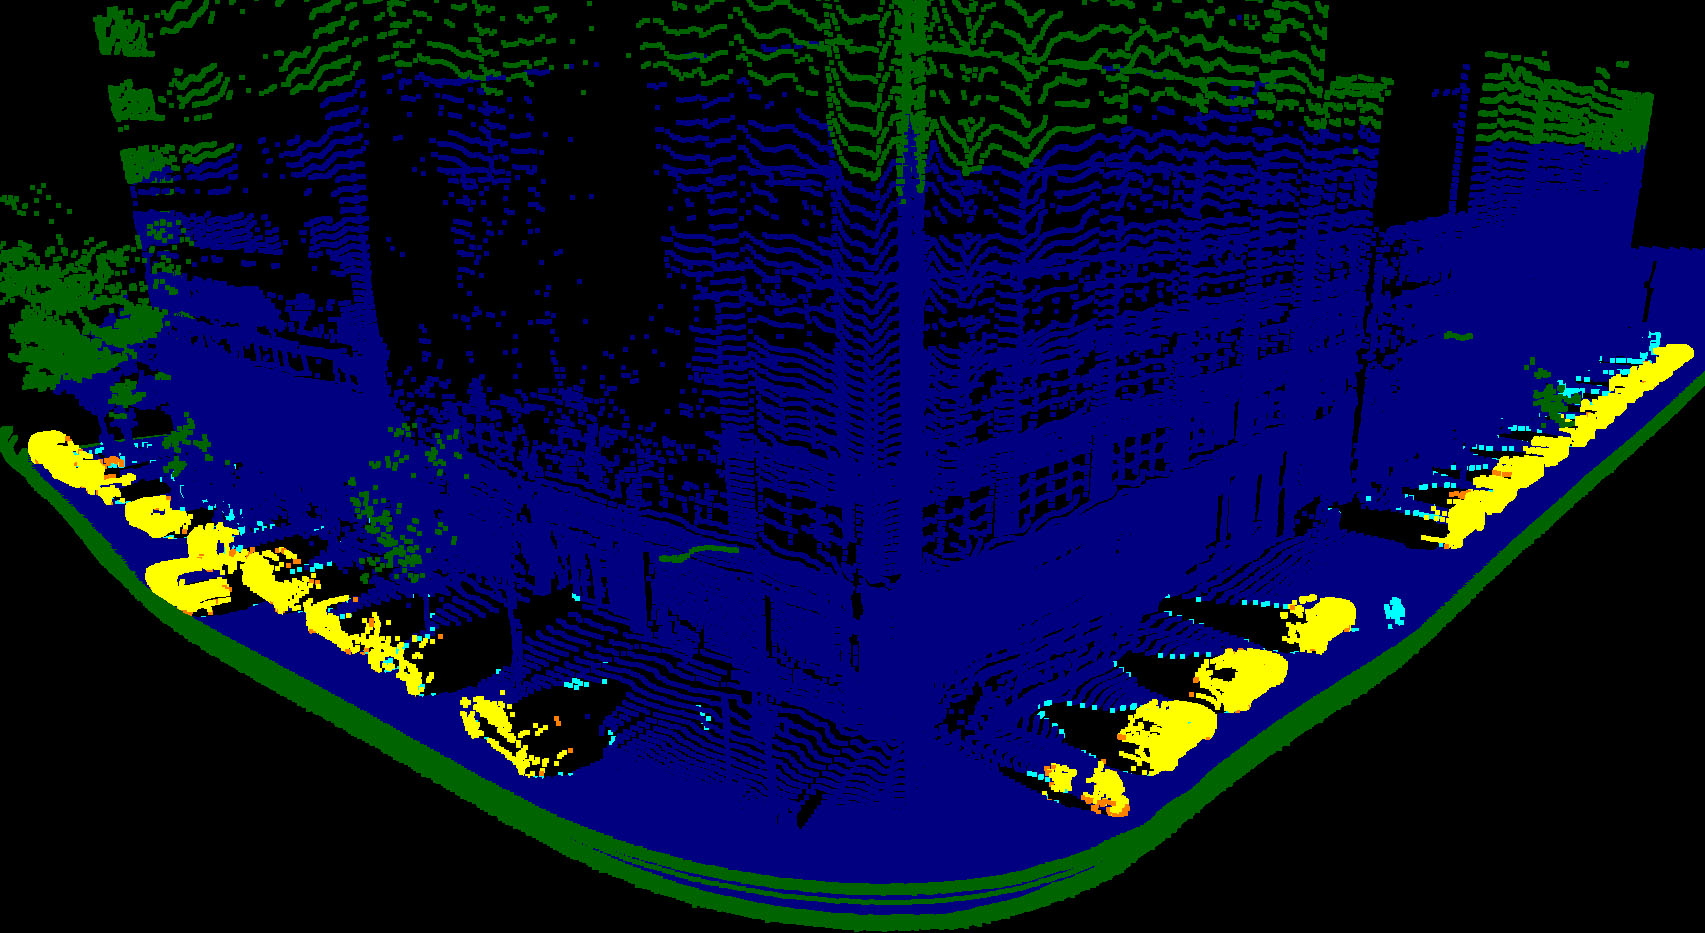
\includegraphics[scale=0.22]{cnn.jpg}
\end{center}
\caption{example of the 3D data from the outdoor urban LIDAR scans\cite{allancnn}.}
 \label{fig:lidar}
 \end{figure}


\begin{figure}[H]
  \begin{center}
      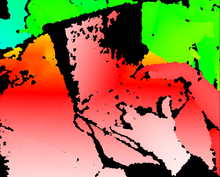
\includegraphics[scale=0.9]{Kinect2-deepmap.png}
\end{center}
\caption{The depth map geenerated by Kinect. The depth map is visualized here using color gradients from white (near) to blue (far)\cite{kinect}}
 \label{fig:kinect}
 \end{figure}
 
 
  
  \begin{figure}[H]
  \begin{center}
      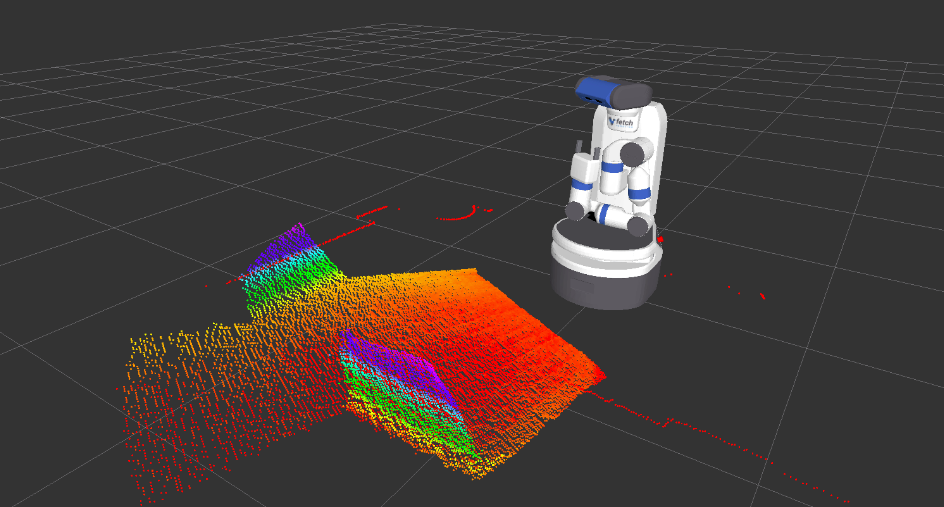
\includegraphics[scale=0.4]{rviz.png}
\end{center}
\caption{The 3D view from the robot of Fetch's perspective.}
 \label{fig:fetch}
 \end{figure}
 
 

\section{Image Classification and Object Detection}
In the computer vision research area, researchers focus on resovle the two main problems: what and where. For the image classification problems, the objective is get what info of this image such as whether this object is a cat or dog. For the object detection problem, the task includes two parts: what and where. For what, the interesting objects will be labelled as a category to infer the what exatly this object is. For the where part, a bounding box will be proposed. This kind of research approach is similar in both 2D and 3D based data.

In this report the papers related to the object classification, object detection and object semantic segmentation for the 2D and 3D objects will be discussed. As most of the state of the art algorithms used for those tasks are based on the deep convolutional neural networks, the important papers related to the deep neural networks will also be discussed in this article.\\
The structure of this article is described bellow: The papers related to the theory part of the deep learning will be discussed in the second session. In the third session, the papers in the 2D object classification will be discussed. In session 4, the 2D object detection papers will be studied. At the same time, an interesting and more challenge related to the 2D image procession or computer vision will be discussed in session 5 which is the 2D object semantic segmentation. In the rest part of this article, the similar tasks in 3D will be discussed as the final goal of this paper review is finding some possible approaches to improve the current 3D computer vision algorithms based on the state of the are 2D computer vision algorithms.\\

\part{Deep Learning Theory}
\subsection{Approximation with Artificial Neural Networks }
In order to build the mathematical theory of the artificial neural networks, several papers are published in the 20 century. The universal approximation theorem with proof is given in \cite{csaji2001}. The theorem claims \cite{csaji2001}  that the standard multilayer feed-forward networks with a single hidden layer that contains finite number of hidden neurons, and with arbitrary activation function are universal approximators in $C(R^m)$.  The universal approximation theorem is one of the important theoretical support for the artificial neural networks. However, at that time as the huge size labeled data sets are not available, the updated algorithms haven't been invented and also the limited computation power, these ideas can not be verified.\\
Inn the year of 1991 Kurt Hornik published a paper \cite{hornik1991} showed that it is not the specific choice of the activation function, but rather the multilayer feedforward architecture itself which gives neural networks the potential of being universal approximators. This is an important contribution which is the foundation for the current state of the art deep learning architecture such as VGG 16  \cite{SimonyanZ14a} and resnet \cite{DBLP:journals/corr/HeZRS15}
The paper of 1986 significantly contributed to the popularisation of BP(Back Propagation) for NNs \cite{Rumelhart1986}, experimentally demonstrating the emergence of useful internal representations in hidden layers. The Back Propagation algorithm is one of the most critical and fundamental algorithm used in the deep neural network. 

%\cite{Schmidhuber201585}
\part{Algorithms developed based on 2D Images}
\section{Image Classification}
The traditional algorithms used for the image classification are nearest neighbor and the SVM. And the features are the flattened pixel values. In th year 1989, the first important application of using the BP(Back Propagation) to well resolve the real life problem from the literature appeared. From this paper, one important structure of the neural network as show in Figure \ref{fig:bpzip} including the layers with filters were introduced. The similar structure is used in the modern neural network structures such as Alex Net\cite{NIPS2012_4824}, VGG 16  \cite{SimonyanZ14a} and resnet \cite{DBLP:journals/corr/HeZRS15}. The basic idea of the convolutional neural network was also introduced here.
\begin{figure}[H]
  \begin{center}
      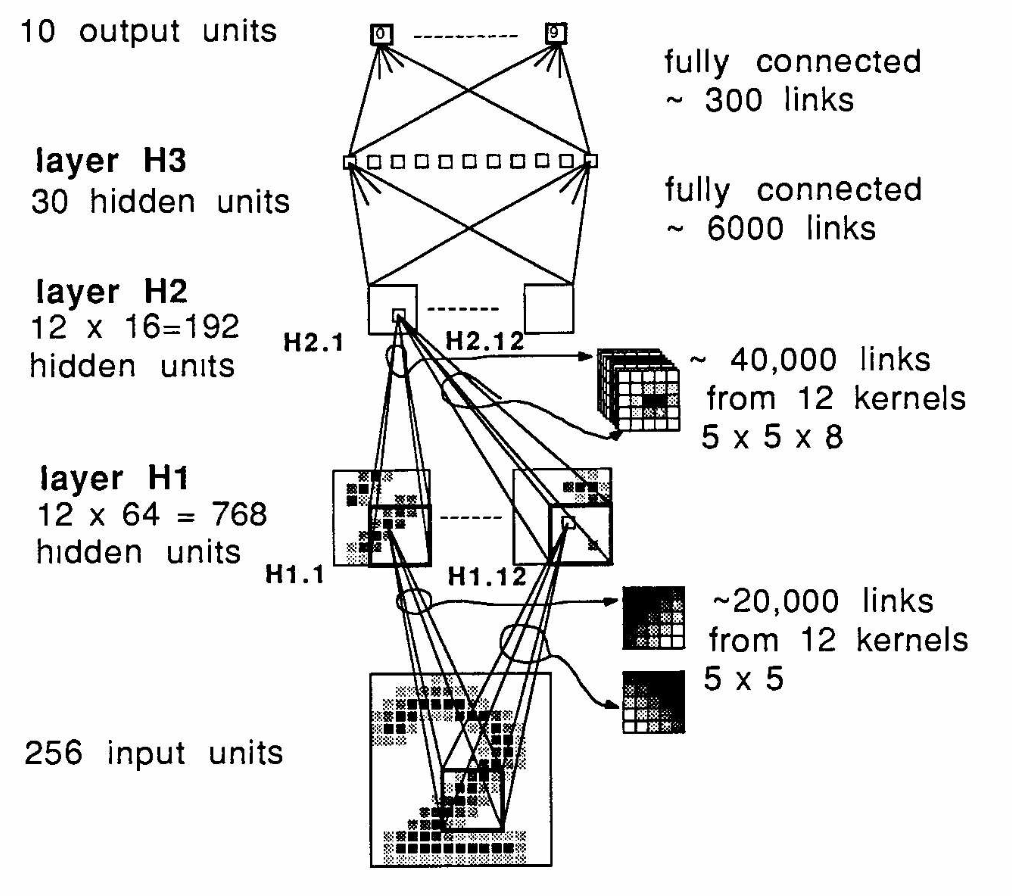
\includegraphics[scale=0.8]{bpzip.png}
\end{center}
\caption{The Neural Network used in \cite{doi:10.1162/neco.1989.1.4.541}.}
 \label{fig:bpzip}
 \end{figure}
One important reason of the taking over of the deep learning algorithms in the computer vsion area is because of the CNN. Another important reason is because of the availablity of the large labelled dataset. As we know, in the machine learning research area, two kinds of learning approaches can be done: supervised learning and unsupervised learning. For the supervised learning algorithms, the labeled data is required to train the algorithm. So the availability of the labeled data will become very important to the development of the supervised learning based algorithms. The ImageNet dataset \cite{imagenet_cvpr09} provides 1.2 million high-resolution labeled images of 1000 categories. This dataset becomes one of the most important datasets related to the object classification.\\
In the ILSVRC-2012 competition, the method following discloused in the \cite{NIPS2012_4824} achieved a winning top-5 test error rate of $15.3\%$, compared to $26.2\%$ achieved by the second-best entry. The outstanding performance of the deep neural network used in this paper brought the focus of both the academic and industry back to the neural network again. In this paper, the CNN network is used and the CNN network structure is illustrated in the Figure \ref{fig:alexnet}. Two GPUs were used to speed up the calculation. Dropout \cite{DBLP:journals/corr/abs-1207-0580} was used here and was proved to be effective to reduce the overfitting problem. The cons of this network is it is a bit complicated and the structure is not so elegant and it will be addressed in the future works by the deep learning researchers. This structure is called as the Alex net to emphasis the unique contribution of the author of this paper.\\


 \begin{figure}[H]
  \begin{center}
      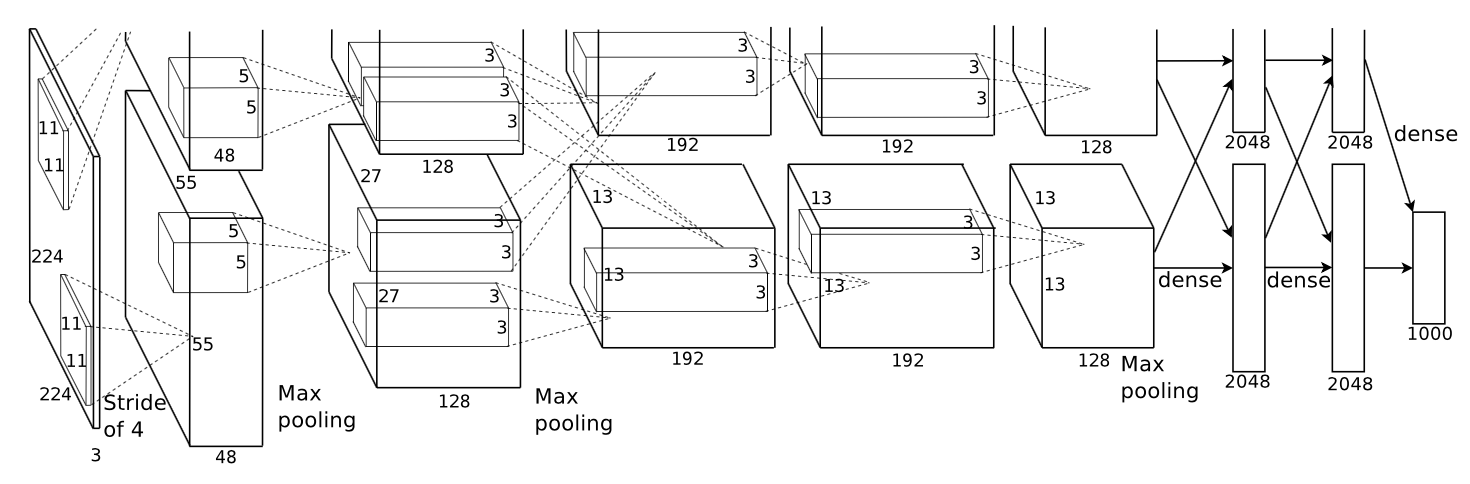
\includegraphics[scale=0.55]{alexnet.png}
\end{center}
\caption{An illustration of the architecture of Alex Net, explicitly showing the delineation of responsibilities between the two GPUs. One GPU runs the layer-parts at the top of the figure while the other runs the layer-parts at the bottom. The GPUs communicate only at certain layers. The network?s input is 150,528-dimensional, and the number of neurons in the network?s remaining layers is given by 253, 440-186, 624-64, 896-64, 896-43, 264-4096-4096-1000\cite{NIPS2012_4824}.}
 \label{fig:alexnet}
 \end{figure}

Two years after the Alex Net, one well orginized VGG network is proposed in paper\cite{NIPS2012_4824}. The structure of this network is very tidy and elegant. Different to the Alex Net\cite{NIPS2012_4824} with different size of the convolutional kernels, in the VGG CNN network\cite{SimonyanZ14a} , only size of 3 by 3 kernels were used for the whole network. At the same time, the trained network weights based on the ImageNet\cite{imagenet_cvpr09} dataset were shared to public. The cons of this model is there are too many parameters and the computation took a long time. Weeks for doing the ImageNet\cite{imagenet_cvpr09}  dataset by using a powerful GPU. \\
This elegant design can also be used in the 3D CNN network to address the 3D object classification problem which will be shown later.\\
 \begin{figure}[H]
  \begin{center}
      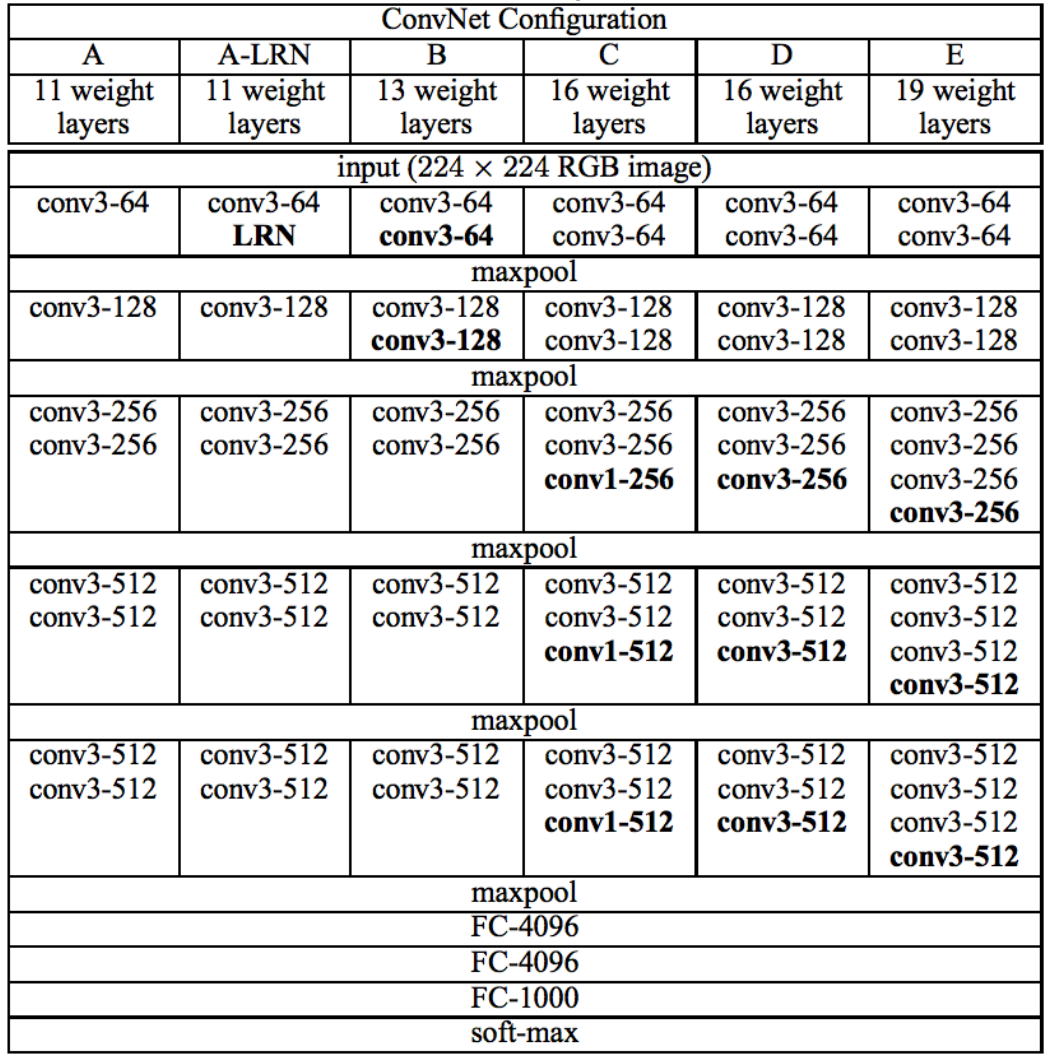
\includegraphics[scale=0.75]{vgg16.png}
\end{center}
\caption{An illustration of the VGG network structure.}
 \label{fig:vgg16}
 \end{figure}

%\subsection{Deep Residual Learning for Image Recognition\cite{DBLP:journals/corr/HeZRS15}}
In the year of 2015, He proposed a new structure of the neural network called resnet\cite{DBLP:journals/corr/HeZRS15} and this new structure increased the layer of the network to more than 100 layers with less parameters than the VGG16 model and better performance. The motivation of this work is trying to find a deeper neural network structure to achieve better performance as the deepest network prior this work is around 20 to 30 layers. The authors had a basic assumption that if more layers are added, the performance should be at least the same as the less layer networks as the new added layers can be designed as the identify layer then the performance can be at least the same. However, the traditional network's performance decreases when the layers increases to a higher level as shown in Figure \ref{fig:resnet}. In order to address this anti-intuitive problem, the authors of this paper designed a deep residual network by adding a short cut between every other layers and finally it shows that this network can achieve a better performance. The problem is addressed. In this paper, the layer of the neural network can goes to 110 layer and have a better performance than the previous state-of-the-art neural network such as VGG16\cite{SimonyanZ14a}, which only has 16 layers neural network. However, as mentioned in \cite{DBLP:journals/corr/HeZRS15}, the parameters used for the 110 layers Resnet is even less than the 16 layers VGG16 network. This seems amazing. However, by reading this article carefully, the main contribution of the reduction of the parameters was using the convolutional network layer instead of the fully connected layer. There is no contribution on the parameters reduction by the Resnet itself.\\
\begin{figure}[H]
  \begin{center}
      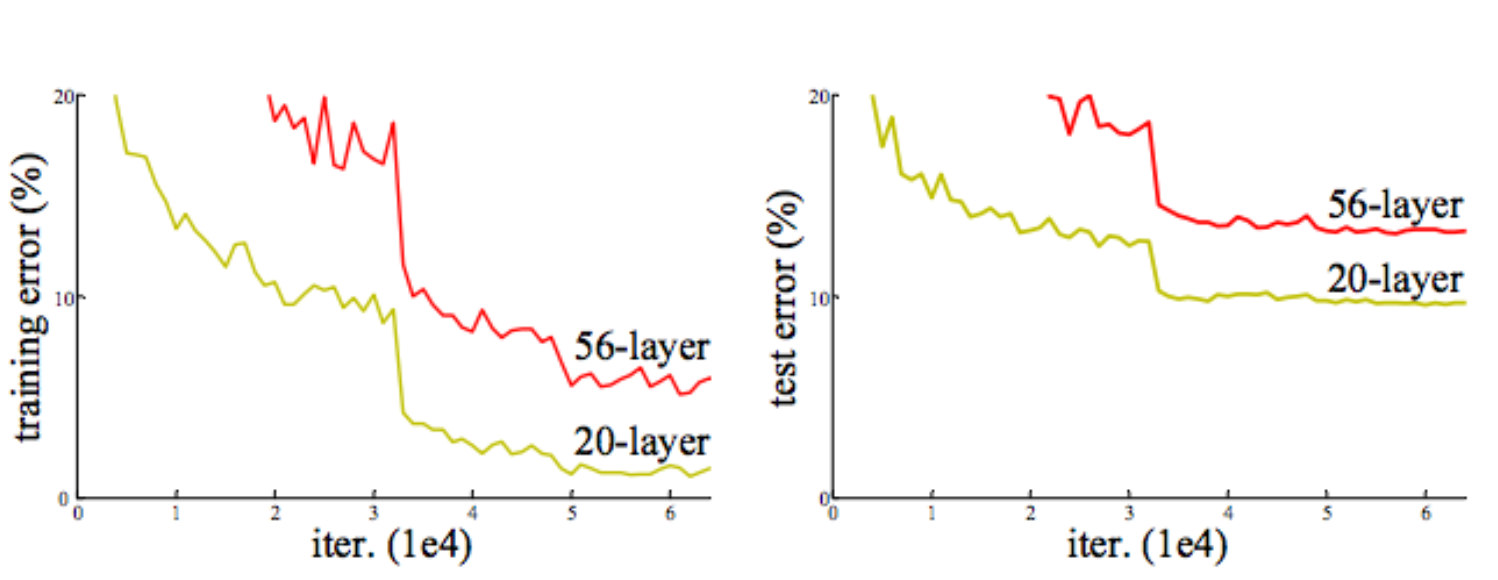
\includegraphics[scale=0.5]{renet1.png}
\end{center}
\caption{An illustration of deep neural networks fails by using the traditional network structure}
 \label{fig:resnet}
 \end{figure}


%%%%%%%%%%%%%%%%%%%%%%%%%%%%%%




\subsection{Batch Normalization: Accelerating Deep Network Training by Reducing
               Internal Covariate Shift\cite{DBLP:journals/corr/IoffeS15}}
The main contribution of this paper as shown in Figure \ref{fig:bp} is it greatly reduced the convergence time for the training process and the BN(Batch Normalization) become one of the standard training step for the deep neural network after the publish of this paper.\\
\begin{figure}[H]
  \begin{center}
      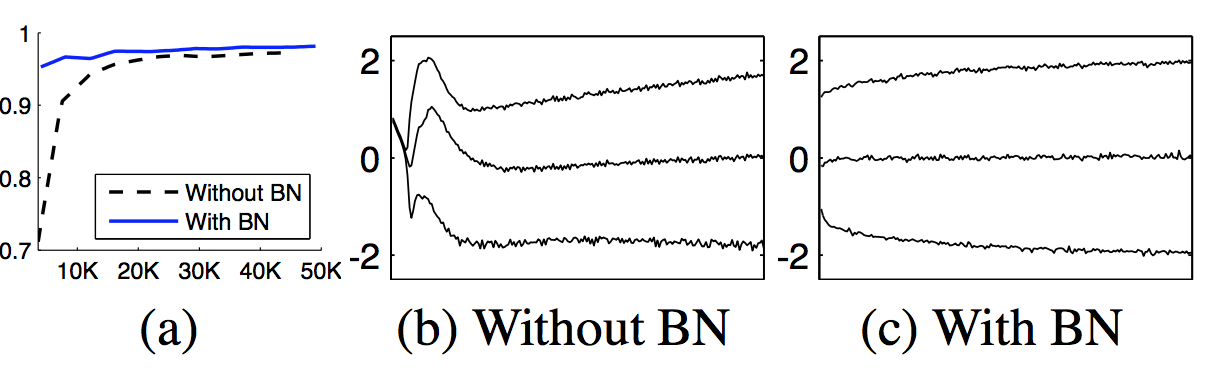
\includegraphics[scale=0.6]{bn.png}
\end{center}
\caption{(a) The test accuracy of the MNIST network trained with and without Batch Normalization, vs. the number of training steps. Batch Normalization helps the network train faster and achieve higher accuracy\cite{DBLP:journals/corr/IoffeS15}. (b, c) The evolution of input distributions to a typical sigmoid, over the course of training, shown as  15, 50, 85th percentiles. Batch Normalization makes the distribution more stable and reduces the internal covariate shift\cite{DBLP:journals/corr/IoffeS15}.}
 \label{fig:bp}
 \end{figure}

%\cite{Schmidhuber201585}
 
\section{Object Detection}

\subsection{Microsoft COCO: Common Objects in Context \cite{DBLP:journals/corr/LinMBHPRDZ14} }
\subsection{Rich feature hierarchies for accurate object detection and semantic
               segmentation\cite{DBLP:journals/corr/GirshickDDM13}}
\subsection{Fast R-CNN\cite{DBLP:conf/iccv/Girshick15}}
\subsection{Faster R-CNN: Towards Real-Time Object Detection with Region Proposal
               Networks\cite{DBLP:conf/nips/RenHGS15}}
\subsection{You Only Look Once: Unified, Real-Time Object Detection\cite{DBLP:journals/corr/RedmonDGF15}}
\subsection{YOLO9000: Better, Faster, Stronger\cite{DBLP:journals/corr/RedmonF16}}

               
\bibliography{jimmy_shen}
\bibliographystyle{ieeetr}
  
 \end{document}
